
\chapter{Systemarkitektur}




\section{Hardware}
\subsection{Design}

\begin{longtabu} to \linewidth{@{}l l l X[l]@{}}
	
	
	Version &    Dato &    Ansvarlig &    Beskrivelse\\[-1ex]
	\midrule
	0.1 &    03-11-2015 &    MB &    Oprettelse \\[-1ex]
	0.2 &    10-11-2015 &    DHC, MB &    Start af skrivning, indsætning af billeder  \\[-1ex]
	0.3 &     &     &     \\[-1ex]
	
	\label{version_Systemark}
\end{longtabu}

Systemets hardware kan illustreres i et BBD. Det ses at nedestående figur at systemet består af fem hardware blokke: software system, forstærker, filter, DAQ og transducer. Disse fem blokke udgør til sammen selve blodtryksmåleren.  
	
\begin{figure}[htb]
	\centering
	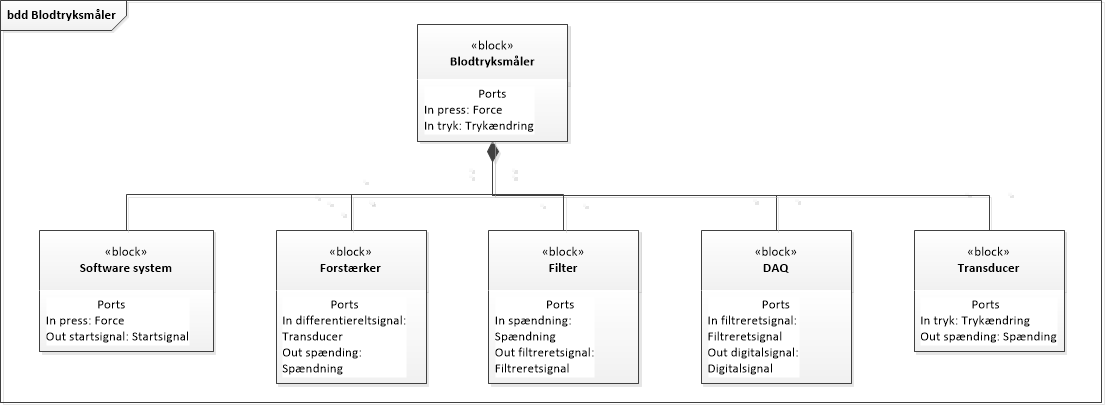
\includegraphics[width=1.0\textwidth]{Figurer/BDD}
	\caption{Block Definition Diagram for hardware}
	%\label{fig:BDD viser blodtrykssystemets hardwaredele, samt sammenhængen mellem disse}
\end{figure}

Ovenstående BDD-diagram fører videre til udarbejdelsen af IBD for hardware komponenterne. I dette diagram vises koblingen mellem de forskellige blokke gennem port forbindelser.  Det ses at signalet starter ved transduceren, hvorefter det bliver behandlet gennem forstærker, filter og DAQ. Til sidste sendes det ind i software systemet, som bliver påvirket at tryk på knapper på GUI. 

\begin{figure}[htb]
	\centering
	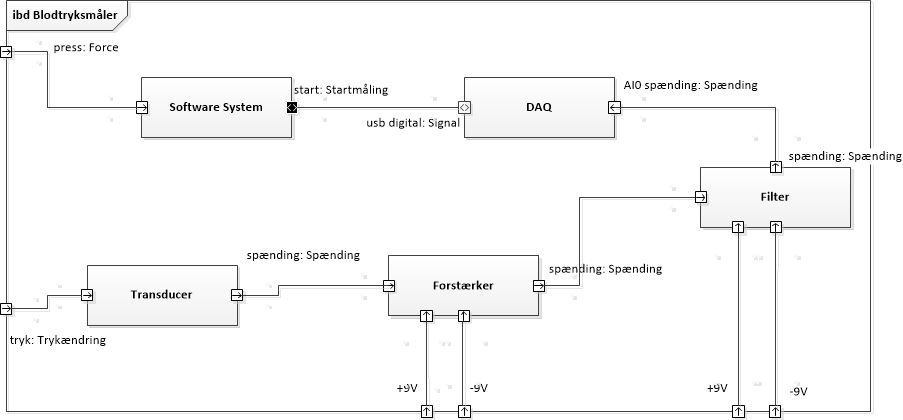
\includegraphics[width=1.0\textwidth]{Figurer/IBD}
	\caption{Infernal Block Diagram for hardware}
	\label{fig:IBD viser koblingen mellem blodtrykssystemets hardwaredele}
\end{figure}

\subsection{Forstærkning}
Transduceren måler en tryk

\subsection{Lavpas}
I projektet skal der laves et 2. ordens lavpasfilter. Dette filter skal være et Salen-Key Buttenworth-filter, med en knækfrekvens på 50 Hz. 

\section{Implementering}
\subsection{Forstærkning}
For at få den rette forstærkning har vi valgt at benytte operationsforstærkeren INA-114. Her kan transduceren sættes på med det differentieret signal. Under opbygning og modultestning vil det differentieret signal blive simuleret af Analog Discovery.
For at få den rette forstærkning ændres der på den "indre" modstand ($ R_g $) til INA114.
  
\subsection{Lavpas}
For at opnå den ønskede effekt i lavpasfilteret, blev det oplyst at $ f_c=50$ Hz, $ R_1 = R_2 $ og $ C_2=680 nF$. Ud fra det udregnes de resterende komponentværdier for filteret.  


\section{Modultest}
\subsection{Forstærkning}
\subsection{Lavpas}
For at teste lavpasfilteret foretages målinger med en sinus, hvor frekvensen variere for hver måling. Derved aflæses fasen, mellem indgang- og udgangssignal, og amplituden for hver måling. 
Ved knækfrekvensen skal fasendrejningen være 90\textdegree. Amplituden skal ændre sig XXX. Dette kan aflæses på billedet Måling for 50 Hz.
Efter knækfrekvensen skal amplituden blive mindre og mindre(går mod nul). På Måling for 60 Hz, kan det ses hvordan amplituden er faldet drastisk efter knækfrekvensen.  \\
\begin{figure}[htb]
	\centering
	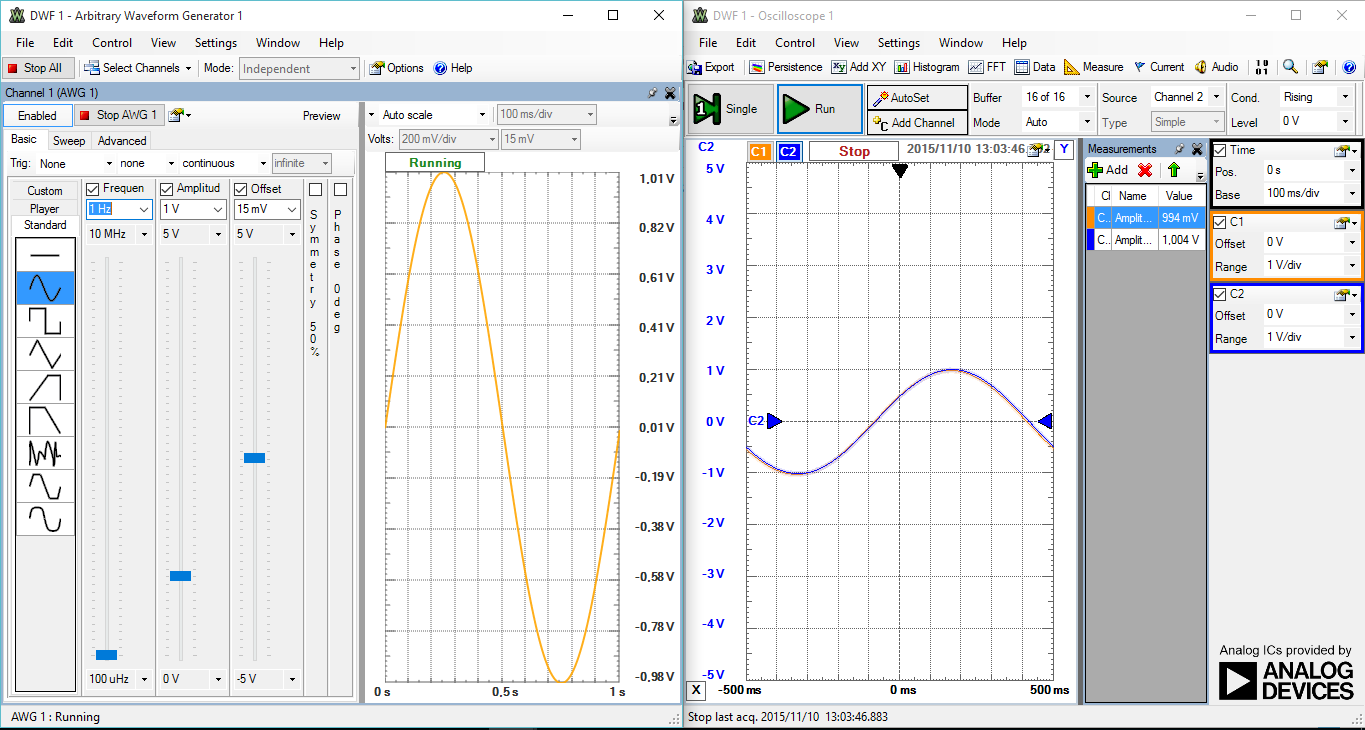
\includegraphics[width=1.0\textwidth]{Figurer/10Hz}
	\caption{Måling for 10 Hz}
	\label{fig:maeling10Hz}
\end{figure}

\begin{figure}[htb]
	\centering
	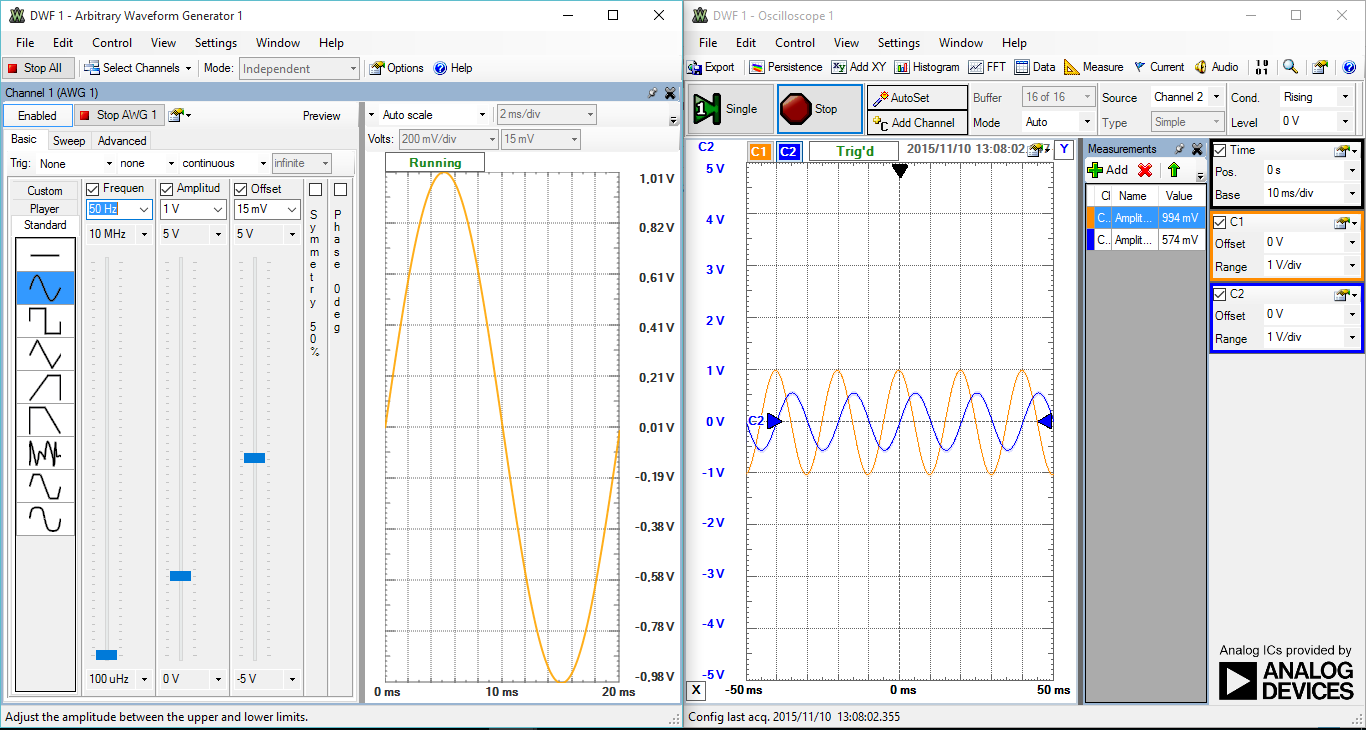
\includegraphics[width=1.0\textwidth]{Figurer/50Hz}
	\caption{Måling for 50 Hz}
	\label{fig:maeling50Hz}
\end{figure}

\begin{figure}[htb]
	\centering
	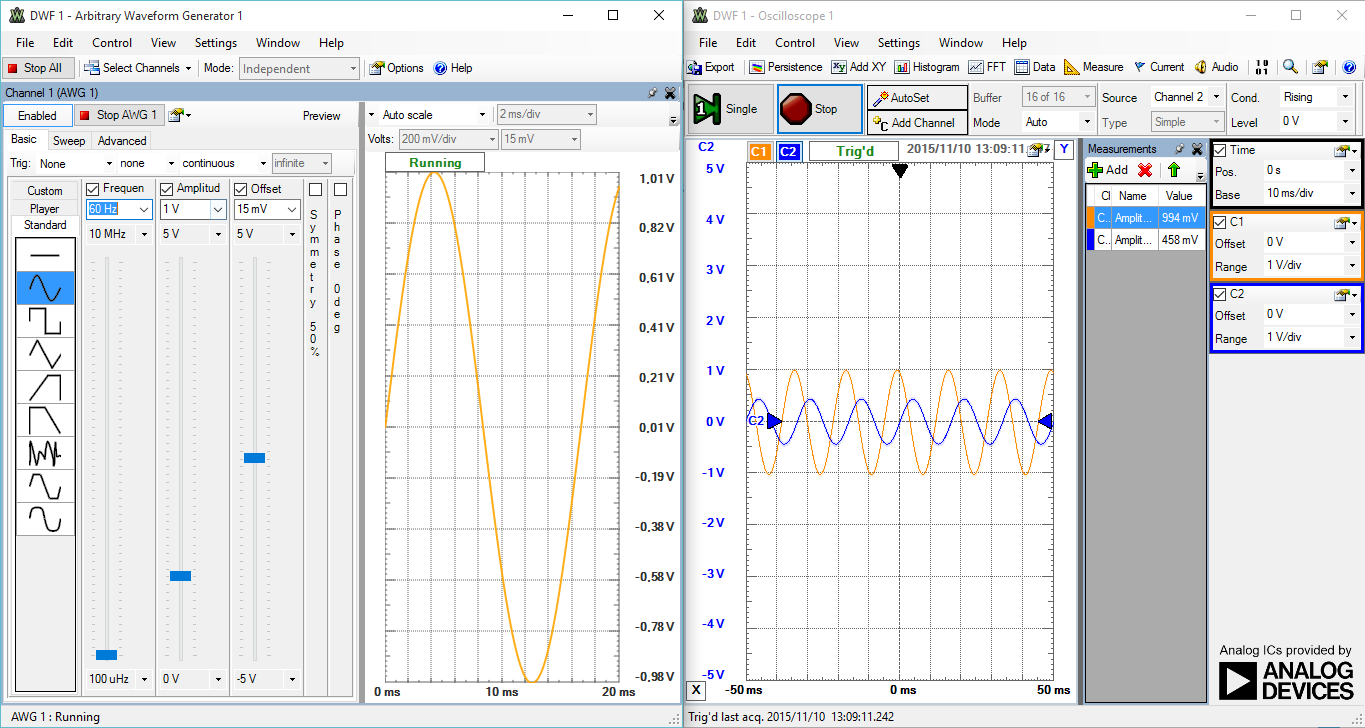
\includegraphics[width=1.0\textwidth]{Figurer/60Hz}
	\caption{Måling for 60 Hz}
	\label{fig:maeling60Hz}
\end{figure}
